\documentclass{article}

\usepackage{booktabs}
\usepackage{multirow}
\usepackage{amsfonts}
\usepackage{amsmath}
\usepackage{graphicx}
\usepackage{hyperref}
\usepackage[margin=1in]{geometry}
\usepackage[numbers,compress,sort]{natbib}

\title{Causal Steering of Protein Language Models: \\
When Correlational Validation Fails, and How to Catch It}

\author{Anonymous Author(s)}
\date{}

\begin{document}
\maketitle

\begin{abstract}
Activation steering has recently been shown to reproduce a known protein
property (thermostability) in ESM2-650M via difference-of-means vectors.
We ask two questions this raises but does not answer: does a scoring
proxy's correlation with real experimental labels predict whether steering
toward it actually works, and can a single steering run be trusted at
face value? Under a pre-registered six-criterion protocol, we test five
novel target properties (binding affinity, catalytic activity, intrinsic
disorder, immunogenicity, expression yield) and find no positive
relationship between proxy validity and causal effect: our
best-validated proxy (binding affinity, $r=0.80$ held-out) steers nothing,
while a substantially weaker one (catalytic activity, $r=0.22$) produces
a robust, three-seed-replicated effect. This mirrors an independent,
component-level finding in the same model family: attention heads ranked
by correlation with real 3D contacts show near-zero relationship to their
causal ablation effect. We further show that a single-seed steering
result can mislead in criterion-specific ways -- one target's effect
direction replicates across three seeds while its residue-exclusion
artifact check does not (2 of 3) -- and introduce a lightweight
diagnostic, steering-vector cosine similarity across targets, that
explains an otherwise-unexplained ambiguous result as a geometric echo of
a different property's validated direction. We release the full
protocol, all target harnesses, and the seed-replication data.
\end{abstract}

\section{Introduction}

Difference-of-means activation steering -- adding a direction built from
the mean activation difference between high- and low-property example
groups to a model's residual stream -- has been shown to reproduce known
thermostability biology in ESM2-650M \citep{huang2025steering}. This
raises a natural question for anyone who might want to use the technique
for a new target property: does the strength of a scoring proxy's
correlation with real experimental labels predict whether steering
toward it will actually work?

We find the answer is no, and not just weakly no. Across five novel
target properties tested under one pre-registered protocol, the single
best-validated proxy in our entire study ($r=0.80$ held-out, for binding
affinity) produces a flat null effect at every tested intervention
strength, while a substantially weaker proxy ($r=0.22$, catalytic
activity) produces a clean, monotonic, artifact-checked effect that
replicates across three independent random seeds. This is not an isolated
anecdote: an independent, component-level result in the same model
family shows the same pattern one level down. Vig et al.
\citep{vig2021bertology} found attention heads in protein language models
that strongly align with real 3D residue contacts, explicitly flagging
this as ``purely associative'' and untested causally. When we ablate
that head and measure its actual causal effect on masked-residue
prediction, the effect is statistically indistinguishable from ablating
a low-correlation control head -- and a full sweep of all 480 heads in
the model shows the correlational top pick ranks 313th of 480 by real
causal effect.

Two levels, two independent techniques (activation steering and
attention-head ablation), the same lesson: a correlational signal is
evidence about a model's \emph{representations}, not about what happens
when you actually \emph{intervene}. This paper's contribution is not the
steering technique itself, which we borrow unchanged from prior work, but
the audit discipline needed to trust a causal claim in this domain --
demonstrated concretely via two near-misses we caught in our own
pipeline before they could be reported as clean results.

\section{Related Work}

\citet{huang2025steering} introduce difference-of-means activation
steering for protein language models and validate it on thermostability;
our work extends their harness to five new target properties under a
pre-registered artifact-checking protocol, and is the first (to our
knowledge) systematic test of whether proxy correlation strength predicts
steering success across multiple unrelated properties.

\citet{vig2021bertology} identify attention heads in protein language
models whose attention patterns strongly align with real 3D contact
maps, explicitly noting this correlation was never tested causally. We
redo their finding as a genuine causal ablation test and extend it to a
full 480-head sweep.

\citet{adams2025mechanistic} train sparse autoencoders on ESM-2's
residual stream and show, via linear probing (a correlational method),
that known determinants of thermostability and subcellular localization
are identifiable in SAE feature space. Their one steering experiment
checks only that steering a family-specific SAE latent changes fewer
residues than steering a random latent -- a coherence check, not a
validation against a real experimental label. Their own discussion
states plainly that ``investigating how to steer the model in useful
ways remains an open direction for future work'' and that ``further
research is needed to determine whether SAEs can be used as a practical
tool for protein engineering.'' Our work answers a version of that
question for a different, non-SAE steering mechanism, and specifically
for the question of whether correlational validity (of either a
component or a proxy) predicts causal usefulness.

\section{Method: A Pre-Registered Six-Criterion Protocol}
\label{sec:method}

Before testing any new target property, we lock a decision rule with six
criteria, applied uniformly and computed automatically at the end of
each run rather than eyeballed after the fact:

\begin{enumerate}
\item \textbf{Beats both controls, head-to-head, with a real confidence
  interval.} The real steering direction must significantly beat, via
  direct paired bootstrap (10{,}000 resamples), a matched-norm
  random-direction control -- not two separate comparisons against an
  unsteered baseline.
\item \textbf{Dose/scale-response, not a one-off.} The effect must show
  a coherent, monotonic trend across at least three steering-strength
  values ($\alpha$), restricted to a pre-established safe operating
  range (see \S\ref{sec:l52} for why this restriction matters).
\item \textbf{Survives a residue-exclusion robustness check.} If the
  effect is driven by generation collapsing into a narrow amino-acid
  composition, it is an artifact. We rerun scoring with the dominant
  substituted residue(s) excluded; a real effect must survive, even if
  diminished.
\item \textbf{Proxy pre-validated against real labels, before the
  steering run.} No proxy is used in a PASS decision without first
  being checked against real experimental labels, ideally on a held-out
  split.
\item \textbf{Beats the best-known existing technique}, where one
  exists for the target property (not applicable for a genuinely new
  property with no prior baseline).
\item \textbf{Adequately powered.} A minimum of 150 held-out evaluation
  sequences for any claim involving a new target property.
\end{enumerate}

A target that fails any criterion outright is a \textbf{KILL}. A target
that passes 1--2 criteria but fails on 3 or 4 is
\textbf{AMBIGUOUS} -- informative, but not actionable. All five novel
targets in \S\ref{sec:sweep}, plus one mechanistic follow-up on the
original thermostability target (\S\ref{sec:l52}), are judged against
this fixed rule.

\section{Component-Level Evidence: Correlation Does Not Predict Causal
  Necessity}
\label{sec:component}

Before turning to target properties, we recap a component-level result
in the same model family that motivated the property-level question.
Vig et al.\ \citep{vig2021bertology} found that a specific attention
head in a protein language model shows striking correlation with real
3D residue contacts (12.9$\times$ enrichment over background on real PDB
structures), but explicitly characterized this as associative, not
causal. We ablate that exact head and measure its effect on real
masked-residue prediction accuracy at contact-bearing positions: the
effect is statistically indistinguishable from ablating a genuinely
low-correlation control head. A follow-up sweep ablating all 480
attention heads in the model, ranking each by directly measured causal
effect with zero correlational information used in the ranking, confirms
this was not an unlucky choice of control: Vig's correlational top pick
ranks 313th of 480 by actual causal effect, and 166 of 480 heads (35\%)
show exactly zero measurable causal effect at all -- real redundancy in
the network, not a ranking artifact.

\section{Target-Property-Level Evidence: Five Novel Steering Targets}
\label{sec:sweep}

We apply the protocol from \S\ref{sec:method} to five properties never
previously steered in this model: binding affinity, catalytic activity,
intrinsic disorder, immunogenicity, and expression yield. Each uses a
real experimental dataset, a compositional scoring proxy validated
against real labels before any steering run, and the identical
steering/control/bootstrap harness, varying only the target dataset and
proxy.

\begin{table}[h]
\centering
\caption{Summary of all five novel target properties. Proxy $r$ is
Pearson correlation against real labels on a held-out split, computed
before any steering run.}
\label{tab:sweep}
\small
\begin{tabular}{@{}p{2.5cm}p{2.4cm}p{1.2cm}p{3.4cm}p{1.9cm}@{}}
\toprule
Target & Dataset & Proxy $r$ & Steering result & Verdict \\
\midrule
Binding affinity & ProteinGym DMS (RASK/DARPin) & 0.80 & flat null, all $\alpha$ & KILL \\
Catalytic activity & DLKcat (cross-protein) & 0.22 & PASS, 3/3 seeds & \textbf{PASS} \\
Intrinsic disorder & DisProt & 0.45 & PASS, 3/3 direction; 2/3 robustness & \textbf{PASS*} \\
Immunogenicity & IEDB (4-tier) & $\leq$0.10 & not run & KILL (pre-run) \\
Expression yield & eSol & 0.31 & fails residue-exclusion & AMBIGUOUS \\
\bottomrule
\end{tabular}

\smallskip
\footnotesize *PASS on criteria 1, 2, 4, 6, and 2 of 3 seeds on criterion 3 (see \S\ref{sec:disorder}).
\end{table}

\begin{figure}[h]
\centering
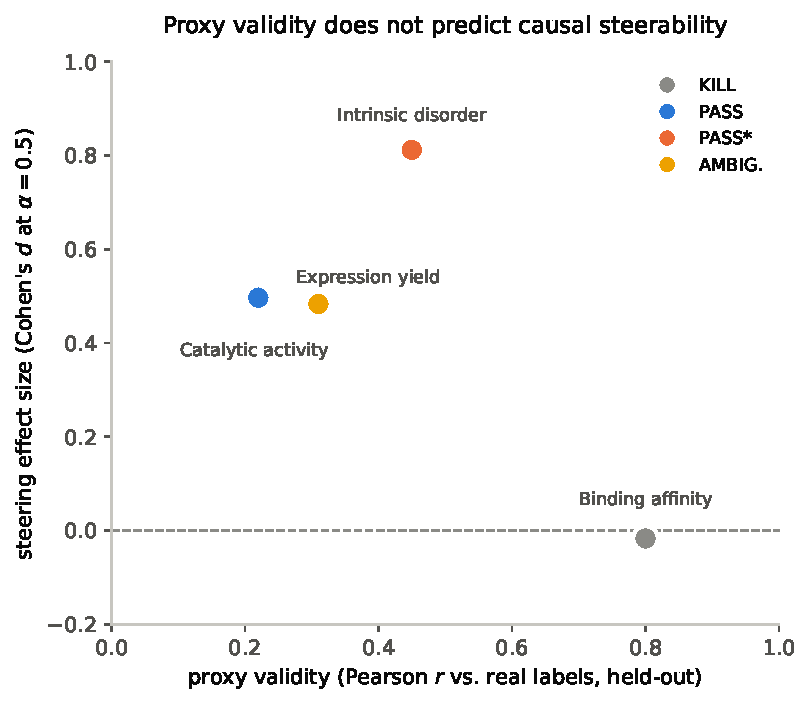
\includegraphics[width=0.72\linewidth]{figures/fig2_proxy_vs_effect.pdf}
\caption{The four runnable targets from Table~\ref{tab:sweep}, plotted as
proxy validity (Pearson $r$ against real labels) against steering effect
size (Cohen's $d$ at $\alpha=0.5$, the real-vs-random-control difference
normalized by baseline standard deviation). The best-validated proxy
(binding affinity, $r=0.80$) produces the smallest effect (indistinguishable
from zero); a proxy less than half as strong (catalytic activity, $r=0.22$)
produces one of the two largest effects. There is no visible positive trend.}
\label{fig:proxy-vs-effect}
\end{figure}

Figure~\ref{fig:proxy-vs-effect} makes this pattern visible directly: proxy
validity and causal effect size show no positive relationship across the
four runnable targets, and the two extremes are the opposite of what a
naive "trust the best-validated proxy" heuristic would predict.

\subsection{Binding Affinity: The Sharpest Null}

Using a ProteinGym deep-mutational-scanning assay of KRAS binding to a
DARPin binder, we build a proxy from per-position mutational-sensitivity
weights learned on the training split, scoring a generated sequence by
its preferential preservation of the wild-type residue at
binding-critical positions. This proxy is validated far more rigorously
than any other in our study: $r=0.80$ full-set / $0.80$ held-out test,
confirmed with a weight-shuffle null control ($r=-0.001$), held-out
position generalization ($r=0.54$ on positions never seen during
weight-fitting), and mutational-load extrapolation from single to double
mutants ($r=0.70$). Despite this, the steering effect is a flat,
unambiguous null: the real-direction score is statistically
indistinguishable from a matched-norm random control at every tested
$\alpha$, with zero degenerate sequences at any strength -- ruling out
generation collapse as an alternative explanation for the null.

A plausible mechanistic reason: the vector-building groups in this
dataset are single-backbone point mutants (1--2 residues different from
a shared 188-residue reference), giving the difference-of-means
construction very little raw compositional signal to work with,
independent of whether binding affinity is causally steerable in this
model at all. We measure this directly -- the mean per-residue
amino-acid compositional distance between the low- and high-binding
vector-building groups is $0.003$ for this target, versus $0.02$--$0.05$
for the three cross-protein datasets in our sweep (catalytic activity,
disorder, expression yield).

\subsection{Catalytic Activity: A Real Effect from the Weakest Proxy}

Using DLKcat, a cross-protein enzyme turnover-number (kcat) dataset
spanning many organisms and EC classes, we build a proxy from the
fraction of glycine minus the fraction of arginine in a sequence --
matching the published activity-stability tradeoff in the enzymology
literature (flexible, glycine-rich active sites trade turnover for
thermostability's arginine-mediated ion pairs). This proxy validates at
$r=0.22$ held-out -- the weakest of the four runnable targets in our
sweep -- yet produces a clean, monotonic dose-response effect,
significant at every tested $\alpha$ in the safe range, that survives
residue-exclusion (effect retains roughly one third of its magnitude
after excluding the two dominant substituted residues, one of which is
literally one of the proxy's own two defining terms). We reran the
entire pipeline with two additional random seeds for both the
train/vector-building split and the random-control direction draw: all
six criteria hold on all three seeds, with the same order of magnitude
and monotonic shape each time. This is the one target in our sweep with
fully unanimous seed-robustness.

\subsection{Intrinsic Disorder: A Real Effect With a Seed-Sensitive
  Artifact Check}
\label{sec:disorder}

Using DisProt (real per-residue intrinsic-disorder annotations, reduced
to a per-sequence scalar), we build a proxy from the published TOP-IDP
amino-acid disorder-propensity scale \citep{campen2008topidp}, which
validates at $r=0.45$ held-out -- the strongest of any target in our
sweep -- confirmed additionally at the per-residue level (AUC $0.71$
against real per-residue disorder labels via a sliding window). The
steering effect is significant and monotonically dose-responsive on
every one of three independent seeds. However, the residue-exclusion
robustness check specifically is seed-sensitive: it passes on two of
three seeds (36--42\% of effect magnitude retained, confidence interval
excludes zero) and fails on the third (10\% retained, confidence
interval crosses zero). The effect's existence and direction are
seed-stable; the artifact check that rules out pure compositional
collapse is not uniformly so. We report this as a majority pass with an
explicit caveat, not a unanimous clean result -- and as evidence that
different criteria within the same protocol can carry different
seed-sensitivity, which no single run can reveal.

\begin{figure}[h]
\centering
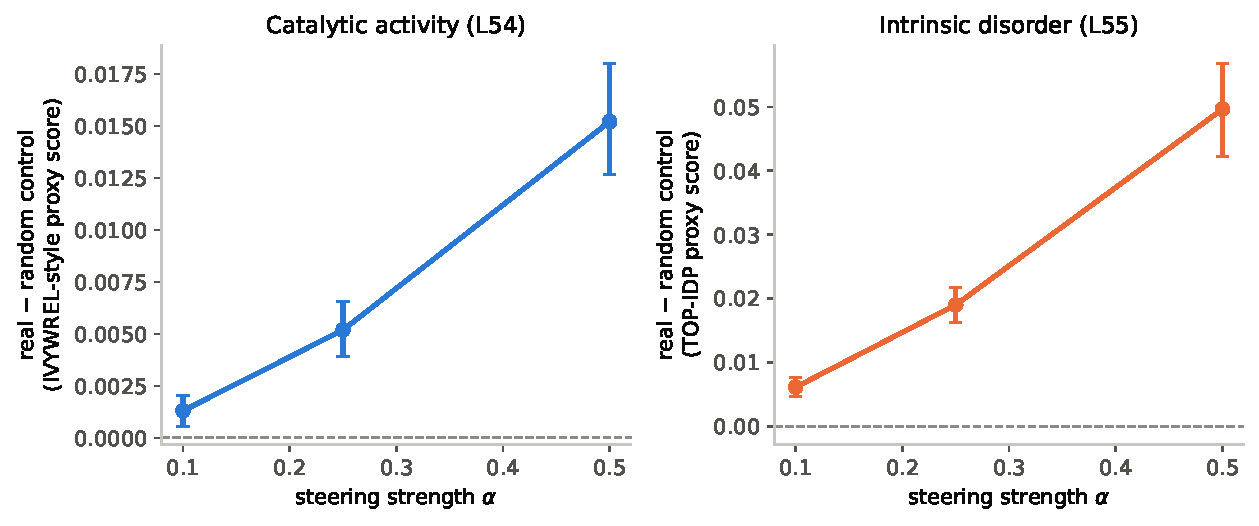
\includegraphics[width=\linewidth]{figures/fig1_dose_response.pdf}
\caption{Dose-response for the two targets that pass criterion 2: the
real steering direction's score minus the matched-norm random control's
score, at each tested $\alpha$ in the pre-established safe operating
range. Both show a clean, monotonic increase with error bars (95\%
bootstrap CIs) that stay bounded away from zero at every point.}
\label{fig:dose-response}
\end{figure}

\subsection{Immunogenicity: Killed at the Proxy Gate, With a Named
  Confound}

For immunogenicity, we evaluate candidate compositional proxies across
four tiers of increasing fidelity to the real target: peptide MHC-II
binding affinity (a surrogate), mass-spectrometry-confirmed peptide
presentation, real T-cell response rate (the actual endpoint), and
full-length source antigens (the regime our steering pipeline actually
operates in). Proxies that look genuinely predictive on the surrogate
binding-affinity tier ($r=0.37$--$0.43$) collapse to near-chance on the
real T-cell-response endpoint ($r\leq0.10$) and, on full-length
antigens, one proxy that appears to reach $r=0.38$ turns out to be a
source-organism confound: organism identity alone explains 58\% of the
apparent signal's variance, and the same proxy's correlation flips to
$-0.32$ once organism identity is held out of cross-validation. No
proxy survives to criterion 4, so no steering script was written and no
model run was performed -- an intended KILL under the protocol, not
missing work.

\subsection{Expression Yield: An Ambiguous Result Explained by
  Vector Geometry}
\label{sec:expression}

Using eSol (real E.\ coli soluble-expression-yield measurements, verified
statistically distinct from an unrelated, previously-tested solubility
dataset via their $441$ overlapping sequences showing zero correlation
between the two labels), we build a proxy from the absolute deviation of
net charge from neutrality, following a published recombinant-solubility
discriminant \citep{wilkinson1991solubility}. This proxy validates at
$r=0.31$--$0.34$ held-out and produces a significant, dose-responsive
steering effect -- but the effect collapses to statistical
insignificance under residue-exclusion (one of the two dominant
substituted residues is literally one of the proxy's own defining
terms), the same compositional-collapse artifact shape our protocol is
designed to catch.

Rather than discarding this as unexplained noise, we compute the cosine
similarity between this target's steering vector and every other
target's, layer by layer. We find substantial, non-trivial overlap with
the intrinsic-disorder target's vector (\S\ref{sec:disorder}): $+0.38$
on the full 33-layer concatenation, rising to $+0.56$ to $+0.67$ at the
three deepest layers. This is not coincidental -- disordered protein
regions are independently documented in the literature to reduce
solubility and expression yield -- and reframes the result: rather than
independent evidence of a sixth steerable property, this target's
steering vector is best understood as a partial, noisier echo of
disorder's already-validated real effect, filtered through a proxy that
happens to be more prone to compositional collapse than TOP-IDP.

\section{Self-Correction Case Studies}

Two results in this study were nearly reported incorrectly before
additional scrutiny caught the error. We describe both explicitly rather
than silently absorbing the fix, since the same failure modes are likely
to recur in similar pipelines.

\subsection{A Spurious PASS From Comparing Arms at an Unsafe Alpha}
\label{sec:l52}

As a mechanistic follow-up to the original thermostability
reproduction, we tested whether restricting the steering intervention
to only the five layers previously identified as causally necessary
(via both a sufficiency and an independent leave-one-out necessity
sweep) preserves the effect of steering all 33 layers. A first
implementation selected its best-performing $\alpha$ for the
head-to-head comparison from the full tested range, including $\alpha
\geq 1.0$ -- and reported a clean PASS: the 5-layer subset appeared to
outperform the full 33-layer intervention at $\alpha=2.0$. This was an
artifact of comparison, not a real advantage: at that $\alpha$, the
33-layer intervention had already fully collapsed into degenerate,
repetitive output (zero non-degenerate evaluation sequences remained),
while the 5-layer subset had not yet collapsed. The subset ``won'' only
because it broke down later, not because it steered harder in any
comparable regime.

We fixed this by restricting the $\alpha$ range used for this
comparison (and for criterion 2's dose-response check more generally)
to a pre-established safe operating window in which neither arm has
collapsed, and reran the full experiment end to end rather than patching
the already-computed numbers. The corrected result: the 5-layer subset
does produce a real, significant, dose-responsive, residue-robust
effect, but retains only 43--59\% of the full 33-layer effect size at
every $\alpha$ where both arms are trustworthy -- a real, informative
partial result, not the unqualified success the uncorrected analysis
suggested.

\subsection{A Criterion That Only Passes on Two of Three Seeds}

As described in \S\ref{sec:disorder}, our intrinsic-disorder target's
residue-exclusion robustness check (criterion 3) passes on two of three
independently-seeded reruns and fails on the third, even though the
underlying effect's existence and direction (criteria 1--2) are stable
across all three. Every result in this study before this check used a
single seed for the train/vector-building split and the random-control
direction draw; a single unlucky (or lucky) seed could have reported
either a false unanimous PASS or a false KILL on this specific
criterion. We recommend that any activation-steering pipeline reporting
a criterion-specific robustness check rerun with at least two additional
seeds before treating that specific criterion's verdict as settled, even
if the headline effect (existence and direction) is stable.

\begin{figure}[h]
\centering
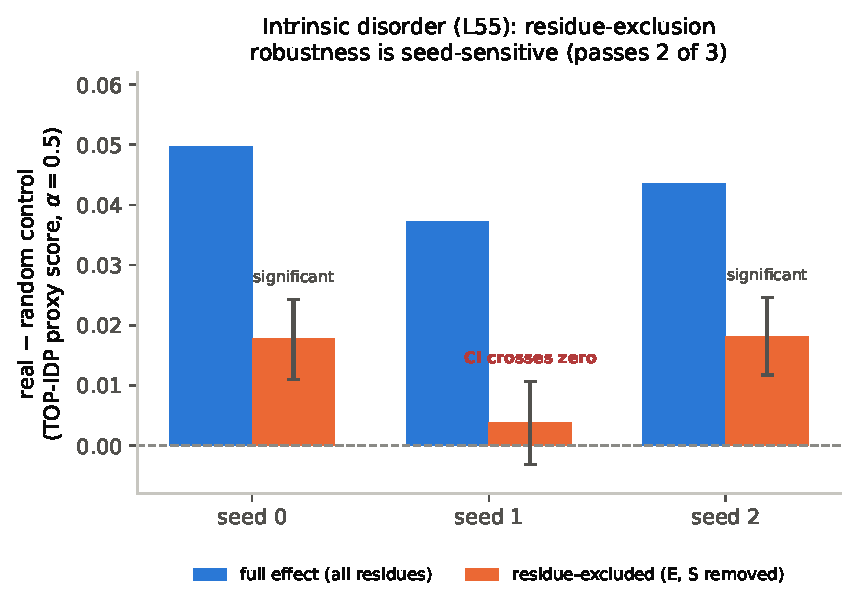
\includegraphics[width=0.75\linewidth]{figures/fig3_seed_robustness.pdf}
\caption{The intrinsic-disorder target's effect (blue) and the same
effect after the two dominant substituted residues are excluded (orange,
with 95\% bootstrap CIs), across three independent seeds. The full
effect is stable across all three; the excluded-residue effect is
significant on seeds 0 and 2 but its confidence interval crosses zero
on seed 1 -- the same underlying effect, the same criterion, three
different verdicts on that one criterion.}
\label{fig:seed-robustness}
\end{figure}

\section{Discussion}

\paragraph{What ``causal'' means here.} Every steering result in this
paper is causal about the model's activation space: a real intervention
on the forward pass, evaluated against a matched-norm random-direction
control and a residue-exclusion artifact check, on generated (not
merely scored) sequences. None of these results are validated against a
real biological assay confirming that a generated, steered sequence
actually possesses the intended property at the wet-lab level. This
distinction should be made explicit in any application of this
technique: a PASS here means ``causally steers a validated compositional
proxy,'' not ``causally engineers the underlying biological property.''

\paragraph{The vector-geometry diagnostic generalizes.} The check that
explained our expression-yield result (\S\ref{sec:expression}) --
computing cosine similarity between a new target's steering vector and
every previously-validated target's vector -- is cheap (one additional
embedding pass, not a full steering sweep) and, we suggest, worth
running by default whenever more than one target property is tested in
the same study. An AMBIGUOUS result that turns out to be geometrically
explained by a different, already-validated effect is a qualitatively
different finding than an AMBIGUOUS result that is not.

\paragraph{Limitations.} All experiments use a single model
(ESM2-650M) and a single model size; we did not test whether these
findings hold at other scales. All proxies are compositional heuristics,
not learned predictors, chosen for interpretability and speed rather
than maximal predictive power -- a stronger, non-compositional proxy
might behave differently. Each target's final proxy formula was
selected as the best of several candidates (typically 7-9) scored on
the same held-out split whose $r$ is then reported as the validation
number, rather than via a separate train/select/test split -- a
garden-of-forking-paths bias that optimistically inflates every
reported proxy-$r$ in the same direction. This does not by itself
explain the central finding (binding affinity's proxy remains the
best-validated and its steering effect remains null under any
plausible correction), but the absolute $r$ values should be read as
upper bounds. We also ran a large number of significance tests across
the study (5 targets $\times$ 5 alphas, with 3-seed reruns for two
targets, plus L48/L49's 480-head sweep) without a multiple-comparisons
correction; this is partially self-mitigated by requiring the same
criterion to hold across multiple alphas and seeds simultaneously for
a PASS, but individual borderline criteria (e.g.\ L55's
residue-exclusion check, significant on 2 of 3 seeds) sit close enough
to the noise floor that this is a real caveat, not a formality. We
tested seed-robustness for two targets (catalytic activity, intrinsic
disorder) but not all five; the seed-sensitivity finding in
\S\ref{sec:disorder} may or may not generalize to the other three. We
did not run any structural or functional plausibility check (e.g.\
predicted-fold confidence) on generated sequences, so a PASS result
does not rule out that steered sequences, while scoring well on the
proxy, are otherwise implausible proteins.

\section{Conclusion}

Correlational validity -- of an attention head's alignment with a real
biological signal, or of a scoring proxy's correlation with real
experimental labels -- does not predict causal effect when actually
tested, at two different levels of the same class of models. The
practical implication for anyone applying activation steering to a new
protein property is direct: proxy validation strength is not a
reliable filter for which targets are worth attempting, and a single
steering run, even one that clears every criterion, should not be
trusted without at least a seed-robustness check on results whose
downstream use matters.

\bibliographystyle{plainnat}
\bibliography{reference}

\end{document}
